\chapter{Javascript}

\section{The Basics}

Javascript heisst eigentlich ECMAScript, welche aktuell in Version 6 vorliegt. Browser unterstützen aber nur Version 5.1. Zudem gibt es noch eine \lstinline|strict|-Version der Sprache. Ist der \lstinline|strict|-Modus aktiviert, muss man z.B. alle Variablen mit \lstinline|var| deklarieren. Um den \lstinline|strict|-Modus zu aktivieren muss man \lstinline|"use strict";| als erste Anweisung des Skriptes oder einer Funktion schreiben.

In Javascript gibt es nur Objekte und keine Klassen. Listing \ref{lst:objekte-deklarieren} zeigt einige Code-Beispiele im Umgang mit Objekten.

\begin{lstlisting}[label=lst:objekte-deklarieren,caption=Objekte deklarieren]
// Objekt durch Object Literal definieren
var bachelorModule = {
	title: "WebApplication Development",
	print: function() { console.log(this.title) }
};
bachelorModule.title;
bachelorModule.print();

// Objekt durch Constructor (immer grossschreiben) deklarieren
function Name(vorname, nachname) {
	this.vorname = vorname;
	this.nachname = nachname;
}

Name.prototype.hello = function(){
	return "Hello" + this.vorname;
}

var name = new Name("Thomas", "Koller");
console.log(name.vorname);
console.log(name.hello());

// Property hinzufügen
name.age = 99;

// Property entfernen
delete name.age;

// nicht definiertes Property
console.log(name.age); // undefined

// nach Property testen
name.hasOwnProperty("vorname"); // true

// Getter / Setter ab ES5
var otherModule = {
	get title() {return "test"},
	set title(value) {}
};
console.log(otherModule.title); // So kann auf Getter zugegriffen werden
\end{lstlisting}

In JavaScript enthält jedes Objekt implizit ein Property dass auf einen Prototypen zeigt. Diese Prototypen sind verkettet, wobei das letzte Objekt der Kette auf den \lstinline|null|-Prototyp zeigt. Wird ein Property im Objekt selbst nicht gefunden, wird die Prototyp-Kette danach durchsucht. Mit Hilfe der Methode \lstinline|Object.getPrototypeOf()| (ES5) kann explizit auf den Prototype zugegriffen werden. Abbildung \ref{fig:prototyp} zeigt wie die Properties \lstinline|vorname| und \lstinline|nachname| beim jeweiligen Objekt sind und die Methode \lstinline|hello()| von beiden Objekten beim Prototyp nachgeschlagen. Der Prototyp selbst, zeigt auf den \lstinline|null|-Prototyp.

\begin{figure}
\centering
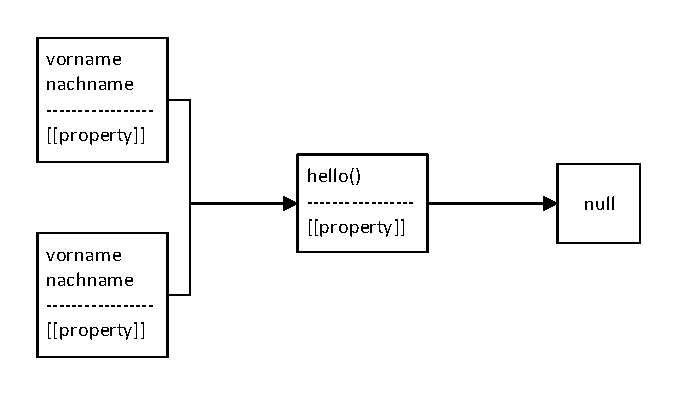
\includegraphics[width=0.7\linewidth]{fig/prototyp}
\caption{Prototyp}
\label{fig:prototyp}
\end{figure}

JavaScript unterstützt JSON von Haus aus. Listing \ref{lst:json} zeigt einige Beispiele zu JSON und Arrays.

\begin{lstlisting}[label=lst:json,caption=JSON]
// JSON.stringify ruft eine Methode toJSON auf (falls diese existiert) und 
// serialisiert das Objekt das zurückgegeben wird
otherModule.toJSON = function(key) {
	var other = {course: this.course, semester: this.semester};
	return other;
}
var otherBachelorModule = JSON.parse(JSON.stringify(otherModule));
console.log(otherBachelorModule);

// Deklaration von Arrays
// Array Literals
var empty = [];
var full = [1,3,8];
var mixed = ["yes", true, 1, 5.0];
var objectArray = [{a:1, b:2}, {a:7,c:15}];

// Array mit new
var another = new Array(); // empty
var oneMore = new Array(5);

// Array Zugriff und Elemente hinzufuegen
var a = ["one"];
console.log(a[0]);
a[1] = "two";
console.log(a.length); // 2

// sparse Array
a[1000] = "thousand"; // Tausendstes Element ist besetzt der Rest ist leer
console.log(a[500]); // undefined

// for loop for sparse arrays
for (var index in a) {
	console.log(a[index]); // one, two, thousand
}

// Weitere Array Methoden -> Buch
// Beispiel reduce (ES5)
var a = [1,2,3,4,5,6];
var sum = a.reduce(function(x,y) {return x+y;}, 0);
console.log(sum); // 21
\end{lstlisting}

In JavaScript sind Funktionen ebenfalls Objekte. Sie erhalten als unsichtbaren Parameter das Keyword \lstinline|this|. Der Wert von \lstinline|this| ist davon abhängig wie die Funktion aufgerufen wird. Listing \ref{lst:methoden-aufruf} zeigt wie Funktionen deklariert und aufgerufen werden. Es gibt vier Möglichkeiten eine Funktion aufzurufen.

\begin{lstlisting}[label=lst:methoden-aufruf,caption=Methoden aufrufen]
// Anonyme Funktion erstellen und an Variable binden
var add = function(a,b) { return a+b; }

// Funktion mit Name an Variable binden (wenn man Funktion rekursiv aufrufen will)
var sub = function sub(a,b) { return a-b; }

// Funktion mit Name ohne an Variable zu binden
function mult(a,b) { return a*b; }

// 1. Funktion mit Name aufrufen
mult(4,5);

// 2. Funktion sofort aufrufen
var fiveToThePowerOfTwo = function(x){return x*x;}(5);
console.log(fiveToThePowerOfTwo);

// 3. Funktion als Literal aufrufen
var aPerson = {
	preName: "Thomas",
	name: "Koller",
	getFullName: function () {
		return this.preName + " " + this.name;
	}
};
console.log(aPerson.getFullName());

// 4. Funktion von anderem Objekt mit apply aufrufen
var dDuck = {
	preName: "Donald",
	name: "Duck"
}

dDuck.getFullName(); // undefined

var donaldsName = aPerson.getFullName.apply(dDuck);
console.log(donaldsName); // Thomas Koller
\end{lstlisting}

In Javascript wird nur pro Funktion ein neuer Scope erstellt. In Listing \ref{lst:scope} werden zwei For-Schlaufen erstellt welche zwei Variablen deklarieren. Eigentlich ist es aber nur eine Variable, weil alle Variablendeklarationen an den Anfang einer Funktion gezogen werden (Hoisting). 

\begin{lstlisting}[label=lst:scope,caption=Scope]
function scopeTest() {
	for(var i = 0; i < 10; i++) {
		console.log(i);
	}
	for(var i = 0; i < 10; i++) {
		console.log(i);
	}
}
// Javascript zieht Variable an den Funktionsanfang (Hoisting)
function scopeTest() {
	var i;
	for(i = 0; i < 10; i++) {
		console.log(i);
	}
	for(i = 0; i < 10; i++) {
		console.log(i);
	}
}
\end{lstlisting}

In JavaScript haben Funktionen Zugriff zum äusseren Scope. Weil auch jede Funktion ein Objekt ist, ist es möglich Closures zu erstellen. Ein Closure kann auch zu einem späteren Zeitpunkt auf seine äusseren Variablen zugreifen, auch wenn dieser Code schon abgearbeitet wurde. Dadurch lassen sich z.B. private Eigenschaften für Objekte erstellen, wie Listing \ref{lst:closure} zeigt.

\begin{lstlisting}[label=lst:scope,caption=Scope]
var myCounter = (function () {
	var value = 0;
	return {
		increment: function (inc) {
			value += inc;
		},
		getValue: function () {
			return value;
		}
	};
}()); // Funktion wird sofort aufgerufen

myCounter.increment(10);
console.log(myCounter.getValue()); // 10
console.log(myCounter.value); // undefined
\end{lstlisting}

Ein Vorteil von Java ist die Objektorientierung und auch die literale Syntax um Objekte zu erstellen. Auch Closures kann man ohne Probleme verwenden. Man sollte darauf achten dass man immer mit \lstinline|===| und nicht mit \lstinline|==|, sonst werden die Werte komisch umgewandelt. Auch die Verwendung von Prototypen und \lstinline|with| sollte man vermeiden. Besondere Vorsicht ist bei globalen Variablen, dem Scope und den Einfügeregeln von Semikolons geboten. Auch das Schlüsselwort \lstinline|typeof| und \lstinline|eval| sind nicht zuverlässig.

\section{Javascript einbinden}
Javascript kann über vier Wege eingebunden werden:
\begin{description}
	\item[Inline] Innerhalb des HTML-Tag \lstinline|<script></script>| kann direkt Javascript-Code geschrieben werden.
	\item[External File] Javascript-Code kann in externe Dateien ausgelagert werden, dafür wird folgends HTML-Tag mit dem Attribut \lstinline|src| benötigt: \lstinline|<script src="something.js"/>|. Der Vorteil der Auslagerung besteht darin, dass Verhalten und Struktur komplett separiert sind und die Wiederverwendung des Javascript-Codes erhöht wird. Ausserdem können die Dateien gecached werden.
	\item[HTML event handler] Beliebiges Javascript kann in spezifischen Attribute in HTML eingefügt werden: \lstinline|<input type="checkbox" name="options" value="giftwrap" onchange="order.options.giftwrap = this.checked;">|. Oft werden einfach Funktionen aufgerufen.
	\item[URL mit javascript: protocol] Wie beispielsweise: \lstinline|<a href="javascript:void(0)">login</a>|.
\end{description}

Die Verarbeitung von Javascript läuft in zwei Phasen ab: In der ersten Phase wird Inline-Javascript ausgeführt und die externen Javascript Files geladen, welche synchron (default), asynchron (\lstinline|<script async>|) oder defered (\lstinline|<script defer>|) ausgeführt werden. Bei async wird der Javascript parallel zum HTML Parsing heruntergeladen und nach dem Download direkt ausgeführt. Bei defer wird der Code auch parallel zum HTML Parsing heruntergeladen aber erst nach dem HTML Parsing ausgeführt (http://www.growingwiththeweb.com/2014/02/async-vs-defer-attributes.html). In der zweiten Phase werden die Event Handler asynchron ausgeführt. 

\section{Timeout \& Interval}
\begin{lstlisting}[label=lst:timeout-interval,caption=Timeout \& Interval]
// Die Funktion f wird nach repetitiv nach Ablauf der Zeit interval mit den Argumenten args ausgeführt.
long setInterval(function f, unsigned long interval, any args...)

// Die Funktion f wird nach Ablauf der Zeit timeout genau einmal mit den Argumenten args ausgeführt.
long setTimeout(function f, unsigned long timeout, any args...)

function myFunction() { alert("Hey!"); }

myTimeout = setTimeout(myFunction, 3000);
clearTimeout(myTimeout);

myInterval = setInterval(myFunction, 1000);
clearInterval(myInterval);
\end{lstlisting}

\section{DOM \& CSS Manipulation}
Mit Javascript wird primär der DOM manipuliert. 

\begin{lstlisting}[label=lst:dom-manipulation,caption=DOM Manipulation]
// Selektion über ID, ID sollte immer indeutig sein
var elt = document.getElementById("quack");

// Selektion über Name, Name muss nicht eindeutig sein
var radiobuttons = document.getElementsByName("favorite_color");

// Selektion über Tag-Name
var firstpara = document.getElementsByTagName("p")[0];
var firstParaSpans = firstpara.getElementsByTagName("span");

// Selektion über CSS-Klasse
var warnings = document.getElementsByClassName("warning");

// Selektion über CSS-Selektoren (HTML5 spezifisch - kennen wir aus jQuery)
var logs = document.querySelectorAll("#log>span");

// DOM-Elemente erzeugen
createElement()
createTextNode()
createComment()
createDocumentFragment() // Hier können vorab grosse Strukturen erstellt werden und auf einen Schlag im Browser dargestellt werden, der Benutzer bekommt nichts mit.

appendChild()
insertBefore()
removeChild()
replaceChild()

// CSS Manipulation
e.style.fontSize = "12pt";
e.style.font-size = "12pt"; // Achtung: Geht nicht!

// Event-Handlers
window.onload = function() {...}
// folgendes ist Equivalent, aber als "schöner" betitelt.
window.addEventListener("load", function(){...}, false);

// Ajax
var request = new XMLHttpRequest();
request.open("GET", "data.json" /* url */);
request.setRequestHeader("Content-Type", "text/plain");
request.send(null /* body */);
request.onreadystatechange = function() {...}

request.onreadystatechange = function() {
	if (request.readyState === 4 \&\& request.status === 200) {
	var type = request.getResponseHeader("Content-Type");
	if (type.match(/^text/)) {
			// do something with request.responseText()
		}
	}
}
\end{lstlisting}

Wir wissen, dass die HTML Struktur in-Memory als DOM repräsentiert wird. Wir können auf die einzelnen Nodes über folgende Attribute zugreifen: parentNode, childNodes, firstChild, lastChild, nextSibling, previousSibling, nodeType, nodeValue, nodeName. Als Beispiel \lstinline|document.childNodes[0].childNodes[1];|. HTML Attribute können wir über Javascript-Properties abfragen: \lstinline|var imgurl = image.src;|. Für alle Nicht-HTML Attribute kann setAttribute, getAttribute, hasAttribute und removeAttribute verwendet werden.

Den Inhalt von Elementen kann auf drei Sichtweisen betrachtet werden. Als Beispiel dient \lstinline|<p>This is a <i>simple</i> document.</p>|. Entweder als HTML-String "<p>This is a <i>simple</i> document.</p>", Plain-Text "This is a simple document." oder als Node-Struktur.

InnerHTML ist Content innerhalb des HTML Element und OuterHTML bedeutet den Inhalt des Element sowie das Element selber.

\section{Typescript}

\subsection{Types}

Typescript hat fast die selben Typen wie Javascript. Zusätzlich kommt noch das Enum, Any und Void hinzu. Das Enum und Void verhalten sich gleich wie in Java. Der Datentyp Any steht für irgendeinen Typ. Man kann Any z.B. verwenden wenn man Benutzereingaben erhält oder Werte von 3rd party libraries. Zudem dient Any der Rückwärtskompatibilität zu normalem Javascript. Der Typ kann natürlich auch weggelassen werden. Listing \ref{lst:types} zeigt einige Codebeispiele.

\begin{lstlisting}[label=lst:typescript-types,caption=Types]
// Nachfolgende Typen sind gleich wie in Javascript
var isDone: boolean = false;
var height: number = 6; // In Typescript gibts auch nur Floating Points Numbers
var name: string = "bob" // Es können Single oder Double Quotes verwendet werden
var list:number[] = [1, 2, 3]; // Ein typisierter Array

// Nachfolgende Typen gibt es in JavaScript nicht
enum Color {Red, Green, Blue};
var c: Color = Color.Green;

var notSure: any = 4;
notSure = "maybe a string instead";
notSure = false; // okay, definitely a boolean

function warnUser(): void {
	alert("This is my warning message");
}
\end{lstlisting}

\subsection{Ambient Declarations}

Damit Typescript problemlos mit herkömmlichem Javascript verwendet werden kann, muss man dem Compiler von Typescript mitteilen, welche Variablen global zur Verfügung stehen. Dieser Mechanismus wird Ambient Declarations genannt. Die Deklarationen für 3rd party libraries werden in einem separaten \lstinline|*.d.ts| abgelegt. Verwendet man beispielsweise die globale \lstinline|process|-Variable von NodeJS, ohne sie vorher zu deklarieren, wird der Compiler eine Fehlermeldung ausspucken. Fügt man aber folgende Anweisung \lstinline|declare var process:any;| ein, lässt sich die Variable verwenden, ohne dass der Compiler reklamiert. Es lassen sich sogar Interfaces von Javascript-Libraries deklarieren. Diese Deklarationen sollte man allerdings mit Vorsicht geniessen, weil man dem Compiler ein Versprechen abgibt, dass diese Variable zur Laufzeit vorhanden ist. Ist sie nicht vorhanden, kann es zu einem Fehler kommen.

\subsection{Functions mit Types und optionalen/default Parametern}

In Typescript lassen sich wie in Javascript benannte oder anonyme Funktionen erstellen. Zusätzlich lassen sich aber die Parameter und der Rückgabewert mit einem Typ versehen. Wenn eine Funktion einer Variable zugewiesen wird, kriegt diese Variable der Typ dieser Funktion. Der Typ einer Funktion setzt sich aus den Typen der Parameter und des Rückgabewerts zusammen. In Typescript ist zudem jeder Funktionsparameter erforderlich. In Javascript hingegen ist jeder Parameter optional. Möchte man optionale Parameter in Typescript haben, muss man diese mit einem Fragezeichen markieren. Zudem kommen die optionalen Parameter immer nach den erforderlichen Parametern. Zudem können auch Default-Parameter mit einem Wert vordefiniert werden. Listing \ref{lst:typescript-functions} zeigt einige Codebeispiele.

\begin{lstlisting}[label=lst:typescript-functions,caption=Functions]
// Variable hat den Typ (x:number, y:number)=>number
var myAdd: (x:number, y:number)=>number = function(x: number, y: number): number { 
	return x+y; 
};

// Optionale Parameter
function buildName(firstName: string, lastName?: string) {}

// Default Parameter
function buildName(firstName: string, lastName = "Smith") {}
\end{lstlisting}

\subsection{Interfaces}

Interfaces in Typescript basieren auf dem \textit{duck typing} Prinzip. Das heisst ein Objekt muss nicht unbedingt \lstinline|implements| verwenden und es muss mindestens die Eigenschaften haben, die vom Interface vorgegeben werden. Das Objekt kann aber auch zusätzliche Eigenschaften haben als das Interface und der Code kompiliert trotzdem. Es ist zudem möglich optionale Attribute bei einem Interface zu deklarieren.

\begin{lstlisting}[label=lst:typescript-interfaces,caption=Interfaces]
interface LabelledValue {
	label: string;
	text?: string; // Optionales Attribute
}

// Funktion welche ein LablledValue nimmt
function printLabel(labelledObj: LabelledValue) {
	console.log(labelledObj.label);
}

// Das Objekt verwendet kein implements hat aber die Eigentschaft label und erfüllt 
// somit das Interface
let myObj = {size: 10, label: "Size 10 Object"};
printLabel(myObj);


interface ClockInterface {
	currentTime: Date;
	setTime(d: Date); // Methode auf Interface definiert
}

// Klasse implementiert Interface
class Clock implements ClockInterface {
	currentTime: Date;
	setTime(d: Date) {
		this.currentTime = d;
	}
	constructor(h: number, m: number) { }
}
\end{lstlisting}

\subsection{Classes}

Klassen in Typescript verhalten sich gleich wie in Java. Es gibt sogar abstrakte Klassen. Allerdings sind alle Instanzvariablen standardmässig \lstinline|public|. Zudem gibt es noch \lstinline|private| und \lstinline|protected|, welche sich auch wie in Java verhalten.

\begin{lstlisting}[label=lst:typescript-classes,caption=Classes]
class Animal {
	name: string;
	constructor(theName: string) { this.name = theName; }
	move(distanceInMeters: number = 0) {
		console.log(`${this.name} moved ${distanceInMeters}m.`);
	}
}

class Snake extends Animal {
	constructor(name: string) { super(name); }
	move(distanceInMeters = 5) {
		console.log("Slithering...");
		super.move(distanceInMeters);
	}
}

class Horse extends Animal {
	constructor(name: string) { super(name); }
	move(distanceInMeters = 45) {
		console.log("Galloping...");
		super.move(distanceInMeters);
	}
}

let sam = new Snake("Sammy the Python");
let tom: Animal = new Horse("Tommy the Palomino");

sam.move();
tom.move(34);
\end{lstlisting}

\subsection{Modules}

In Typescript gibt es ein Modulsystem. Variablen, Funktionen usw. in einem Modul sind nicht mehr global sichtbar, ausser die welche explizit mit \lstinline|export| öffentlich gemacht wurden. Möchte man etwas von einem anderen Modul konsumieren muss man es mit dem \lstinline|import| in den eigenen Code einbinden. Jede Datei welche ein \lstinline|export| oder \lstinline|import| beinhaltet wird als Modul deklariert. 

\begin{lstlisting}[label=lst:typescript-modules,caption=Modules]
export const numberRegexp = /^[0-9]+$/;

export class ZipCodeValidator {
	isAcceptable(s: string) {
		return s.length === 5 && numberRegexp.test(s);
	}
}

import { ZipCodeValidator } from "./ZipCodeValidator";

let myValidator = new ZipCodeValidator();
\end{lstlisting}